\documentclass[11pt]{article} % do not change this line
\input{BigDataStyle.txt}      % do not change this line
\usepackage[hidelinks]{hyperref}
\usepackage[export]{adjustbox}
\usepackage{amsmath,amsfonts,amssymb,amsthm,latexsym,graphicx,url,bookmark,enumitem}

\emergencystretch=5mm
\tolerance=400
\allowdisplaybreaks[4]

\theoremstyle{plain}
\newtheorem{theorem}{Theorem}[section]
\newtheorem{proposition}[theorem]{Proposition}
\newtheorem{corollary}[theorem]{Corollary}
\newtheorem{lemma}[theorem]{Lemma}
\newtheorem{problem}[theorem]{Problem}

\theoremstyle{definition}
\newtheorem*{remark}{Remark}

\title{Machine Learning for Investor Behaviours on Cryptocurrencies}
\author{Chengkai Lu}

\newcommand{\Programme}{Data Science and Analytics with a Year in Industry}

\begin{document}
\maketitle

\declaration

\begin{abstract}
  Your abstract goes here.
\end{abstract}

\listoffigures
\listoftables

\clearpage

\section{Introduction}
\subsection{Motivation}
\subsection{Aims And Objectives}
\subsection{Project Structure}
\subsubsection{Technologies}
\subsubsection{Programme Structure}
\subsubsection{Report Structure}

\section{Background Research}
\subsection{Correlation Analysis}

In statistics, covariance\eqref{eq:1} defines the variability between two individual attributes, which means the level of influence from one feature to another. The numbers correspond to similarity/dissimilarity of the two variables. Positive numbers represent a similar behaviour between them, and vice versa\cite{wiki/cov:2018}.

{
  \begin{equation}
    \label{eq:1}
    {\operatorname {cov} (X,Y)=\operatorname {E} [(X-\mu _{X})(Y-\mu _{Y})]}
  \end{equation}

  \footnotesize
  where:
  \begin{itemize}[label=-, leftmargin=4em, itemsep=0.1em]
    \item ${E}$ is the expectation
    \item ${X, Y}$ are vectors of all the samples
    \item $\operatorname {cov}$ is the covariance
    \item ${\mu}_{X}$ is the mean of X
    \item ${\mu}_{Y}$ is the mean of Y
  \end{itemize}
}

However, if we want to measure the strength of the linear relationship in between, covariance is not enough. We also need to consider the variance in each feature to tell whether the linear relationship is strong. In this case, the correlation was introduced. Correlation is a normalised form of covariance. It restricts the numbers to a certain range which shows how strong the relationship is. The most commonly used correlation coefficient is Pearson correlation coefficient\eqref{eq:2}. it is calculated by considering the standard deviation of both groups. This can ensure that dispersion of either attribute does not interfere our identification on the strength of mutual linear relationships\cite{wiki/pcc:2018}.

{
  \begin{equation}
    \label{eq:2}
    \rho _{X,Y}={\frac {\operatorname {cov} (X,Y)}{\sigma _{X}\sigma _{Y}}}
  \end{equation}

  \footnotesize
  where:
  \begin{itemize}[label=-, leftmargin=4em, itemsep=0.1em]
    \item ${\rho}$ is the Pearson correlation coefficient
    \item ${X, Y}$ are vectors of all the samples
    \item $\operatorname {cov}$ is the covariance
    \item ${\sigma}_{X}$ is the standard deviation of ${X}$
    \item ${\sigma}_{Y}$ is the standard deviation of ${Y}$
  \end{itemize}
}

The value of Pearson correlation coefficient is always between -1 and 1. A positive number means a positive linear correlation, and a negative number means a negative linear correlation. The closer the number towards the extremes, the stronger the relationship is. If the number is 0, it means there is no linear correlation among the pair\eqref{eq:3}.

\begin{equation}
  \label{eq:3}
  \text{relationship} = 
  \begin{cases} 
    \text{total positive linear correlation} & \text{if } \rho = 1 \\
    \text{positive linear correlation} & \text{if } \rho > 0 \\
    \text{no linear correlation} & \text{if } \rho = 0 \\
    \text{negative linear correlation} & \text{if } \rho < 0 \\
    \text{total negative linear correlation} & \text{if } \rho = -1
  \end{cases}
\end{equation}

\subsubsection{Correlation Matrix}

Given a set of data with multiple attributes, we may want to tell people how these attributes interact with each other. In addition, the result of analysis, especially in a simple regression, may not be reasonable when those features are highly dependent.

To achieve this, we can create a matrix which contains all the correlation coefficient calculated from the expanded equation\eqref{eq:3} with a set of given samples.

{
  \begin{equation}
    \label{eq:4}
    {\rho_{xy}={\frac {\sum _{i=1}^{n}(x_{i}-{\bar {x}})(y_{i}-{\bar {y}})}{{\sqrt {\sum _{i=1}^{n}(x_{i}-{\bar {x}})^{2}}}{\sqrt {\sum _{i=1}^{n}(y_{i}-{\bar {y}})^{2}}}}}}
  \end{equation}

  \footnotesize
  where:
  \begin{itemize}[label=-, leftmargin=4em, itemsep=0.1em]
    \item ${\rho}$ is the Pearson correlation coefficient
    \item ${n}$ is the sample size
    \item $x_{i}, y_{i}$ are the single samples indexed with i
    \item ${\bar {x}}={\frac {1}{n}}\sum _{i=1}^{n}x_{i}$ (the sample mean)
    \item ${\bar {y}}={\frac {1}{n}}\sum _{i=1}^{n}y_{i}$ (the sample mean)
  \end{itemize}
}

A correlation matrix is a symmetirc matrix to its main diagonal. The values on the main diagonal always equal to 1 because the attributes are fully dependent on themselves. Table \ref{table:cormat} gives an example of how a correlation matrix looks like.

{
  \begin{table}[h]
    \centering
    \begin{tabular}{|c|c c c c c|}
      \hline
      Features & f1 & f2 & f3 & f4 & f5 \\ [0.5ex]
      \hline
      f1 & 1 & 0.74 & -0.38 & 0.12 & 0.43 \\ 
      \hline
      f2 & 0.74 & 1 & 0.26 & 0.88 & -0.57 \\
      \hline
      f3 & -0.38 & 0.26 & 1 & 0.61 & 0.59 \\
      \hline
      f4 & 0.12 & 0.88 & 0.61 & 1 & -0.22 \\
      \hline
      f5 & 0.43 & -0.57 & 0.59 & -0.22 & 1 \\ 
      \hline
    \end{tabular}
    \caption{Correlation Matrix}
    \label{table:cormat}
  \end{table}
}

\subsection{Dimensionality Reduction}

It is always challenging to analyse a dataset with high-dimensional data points. Due to the curse of dimensionality, which was discovered by Richard Ernest Bellman in 1961, higher dimensional space increases the difficulties of analysing and organising data exponentially\cite{wiki/cod:2018}. Especially in machine learning, given a certain number of samples, the accuracy of predictions on these samples will increase followed by the rising dimensions to a peak but then gradually drop. This is known as Hughes phenomenon\cite{hughes/itoit:1968}. Figure \ref{fig:hughes} shows how the dimensionality influence the accuracy of predictions.

\begin{figure}[h]
  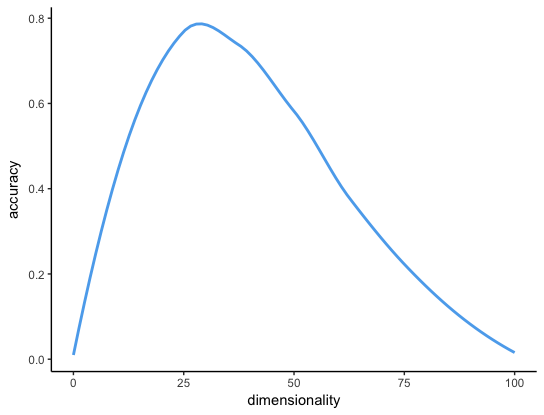
\includegraphics[width=0.8\linewidth, center]{resources/dimensionality.png}
  \caption{Hughes phenomenon}
  \label{fig:hughes}
\end{figure}

In order to reduce the dimensionality, there are two approaches can be implemented:
\begin{itemize}
  \item Feature Selection: To select a subset that is more informative or relevant among all the attributes\cite{hastie/etal:2009}.
  \item Feature Extraction: To generate new features from the initial attributes of existing data\cite{wiki/fe:2018}.
\end{itemize}

The reasons and benefits of executing dimensionality reduction can be summarised as follow:
\begin{enumerate}
  \item Computational efficiency: Fewer features mean less computation on dissimilarity between pairs of data points and lower arithmetic complexity. It also implies less storage usage as the variables in each sample decrease.
  \item Statistical generalisation: By removing noise or irrelevant information from the inputs for building models, the prediction rules can be more general among the datasets.
  \item Better explanation: Visualising a lower dimensional space is much easier. We can effortlessly illustrate the structure of data when the dimension is lower than 3. Higher dimensional space will be more challenging to visualise, explain and comprehend.
\end{enumerate}

\subsubsection{Principal Component Analysis}

Principal component analysis (PCA) is a method for feature extraction. 

\subsection{Clustering}

Clustering, cluster analysis or data segmentation is a non-parametric algorithm in the subtree of unsupervised learning. It is used to separate data into different groups using their natural dissimilarities. Unlike supervised learning, this type of learning algorithms does not have any indicator for assessing the quality of results, and this means that it does not have any meaning or objective itself. Instead, it discovers the distribution of data and uses the definition given by people who have the specific domain knowledge. By giving the rules for partitioning data self-defined meanings, useful information can be obtained and utilised in different domains\cite{hastie/etal:2009}.

Generally, 

\subsubsection{K-means Clustering}

\subsection{Recurrent Neural Network}
\subsubsection{Long Short-Term Memory}

\section{K-means Clustering on Price Fluctuations}
\subsection{Data Prepocessing}
\subsubsection{Data Formats}
\subsubsection{Normalisation}
\subsection{Data Analysis}
\subsubsection{Shifting Along Timeline}
\subsubsection{Model Training}
\subsection{Result}

\clearpage

\section{LSTM on Highest/Lowest Nextday Growth Prediction}
\subsection{Data Prepocessing}
\subsubsection{Data Formats}
\subsubsection{Normalisation}
\subsubsection{Training Set and Validation Set}
\subsection{Data Analysis}
\subsubsection{Activation Functions}
\subsubsection{Parameters}
\subsubsection{Regularisation}
\subsubsection{Loss Function}
\subsubsection{Model Training}
\subsection{Result}
\subsubsection{Back Test}

\section{Performance}
\subsection{K-means Clustering}
\subsection{Long Short-Term Memory}

\section{Conclusion and Evaluation}
\subsection{Visualisation}
\subsection{Further Work}

\section{Appendix}
\subsection{Programme Usage}

\bibliographystyle{plain}
\bibliography{bibliography}
\end{document}
